\section{Method}

In order to develop an adequate model of baseline brainstorming performance in crowd marketplaces, it was necessary to establish a corpus of data. Over the course of four months we repeatedly collected responses to brainstorming tasks. Throughout the experimental process, particular aspects of the experimental design remained fixed.

The independent variables of interest were \emph{brainstorming problem} and \emph{number of ideas requested}.

Participants were recruited from Amazon's \emph{Mechanical Turk} (CITE), and were restricted to residents of the United States for a baseline expectation of english language comprehension and cultural familiarity. Mechanical Turk is an online marketplace in which members receive financial reward for completing \emph{Human Intelligence Tasks}, or HITs.

HITs were placed on the marketplace for each \emph{number of ideas requested} condition, with proportional rewards. Participants could accept at most one HIT in each of these conditions.

Upon accepting a HIT, participants were randomly assigned into a \emph{brainstorming problem} condition. We ensured that participants completing multiple HITs are not exposed to the same brainstorming task twice.

\subsubsection{Design Concerns}
Workers choose which HITs to complete, thus self-selection bias is a reasonable concern. This bias is also present in real-world HIT choice behaviour. 

Upon accepting a HIT, participants were asked to give consent and informed that they could leave the study at any point without financial consequences. In regular online task markplaces, common practice would restrict workers from submitting a HIT as complete unless all responses were given. This is a threat to external validity.

\subsection{Task}

The brainstorming task is a form in a standard web browser. Participants are presented with a brief overview of the tenets of brainstorming, are presented a problem, and must enter some number of ideas to resolve the problem within an 18 hour period.

At the beginning of the form is a brief introduction to brainstorming, with a paraphrase of Osborne's four rules of brainstorming (CITE). These rules were manipulated to make sense within the constraints nominal brainstorming over the web medium. The rules, as displayed to the participants:

\begin{enumerate}
\item There are no bad ideas. Don't criticise your choices.
\item Wild ideas and building off of old ideas are okay.
\item Quantity of ideas is prioritized.
\item Combinations of ideas count as new ideas.
\end{enumerate}

The brainstorming task is below this, followed by a series of text entry inputs numbered through to the total number of ideas requested. Figure X (FIG) is an example of a typical task. We place a larger free text area at the bottom of the list where participants could enter any additional ideas.

\subsection{Pilots and Question Selection}

With this basic design in hand, we ran several pilots and experiments. In early pilots, we used classic problems from psychology literature on brainstorming, including the "thumb problem" and "broom problem" (CITE). Early results from brainstormers were unsatisfying and wildly divergent. We identified three key traits problems needed in order to evaluate them for creativity:

\begin{enumerate}
\item They must require creativity to resolve. Obvious answers do not satisfy the problem.
\item They must be problems that participants on Mechanical Turk would have the expertise to solve.
\item They must have an associated success metric.
\end{enumerate}

The primary researcher and two additional researchers familiar with crowd marketplace brainstorming tasks brainstormed a large variety of potential problems. These problems were iterativelly culled and refined over a series of further pilots until the above goals were felt to be achieved. This resulted in the following four questions, as presented to the participants:

\begin{enumerate}
\item \textbf{Charity}

The Electronic Frontier Foundation (EFF) is a nonprofit whose goal is to protect individual rights with respect to digital and online technologies. For example, the EFF has initiated a lawsuit against the US government to limit the degree to which the US surveils its citizens via secret NSA programs. If you are unfamiliar with the EFF and its goals, read about it on its website (https://www.eff.org) or via other online sources (such as Wikipedia).

Brainstorm N \emph{new} ways the EFF can raise funds and simultaneously increase awareness. Your ideas \emph{must be different from their current methods}, which include donation pages, merchandise, web badges and banners, affiliate programs with Amazon and eBay, and donating things such as airmiles, cars, or stocks. See the full list of their current methods here: https://www.eff.org/helpout. Be as specific as possible in your responses."

\item \textbf{Mechanical Turk}

"Mechanical Turk currently lacks a dedicated mobile app for performing HITs on smartphones (iPhone, Androids, etc.) or tablets (e.g., the iPad).

Brainstorm N features for a mobile app to Mechanical Turk that would improve the worker's experience when performing HITs on mobile devices. Be as specific as possible in your responses.

\item \textbf{MP3}

Many people have old MP3 players or MP3 players that they no longer use. Please brainstorm N uses for old MP3 players/MP3 players. Assume that the devices' batteries no longer work, though they can be powered via external power sources. Also be aware that devices may \emph{not} have displays. Be as specific as possible in your descriptions.

\item \textbf{Forgot Name}

Imagine you are in a social setting and you have forgotten the name of somebody you know. Brainstorm N ways you could learn their name without directly asking them. Be as specific as possible in your descriptions.

\end{enumerate}

Classic brainstorming procedure asks for as many ideas as possible in a period of time. We instead asked participants for a specific number of responses: 5, 10, 20, 50, 75 or 100.

This decision was motivated by our early experience asking respondants to simply come up with "as many ideas as possible" in a generous time frame. Over N respondents, we received a mean of N ideas (std N), despite giving a financial reward N times that of any of our explicitly numbered conditions. This unlimited condition provided a great deal of leeway for participants to "game the system", and receive the full reward with very little work, so we dropped the condition.

\subsection{Experiment}

With the above problem set and the previously outlined task design (SEC), we collected responses. We chose 6 \emph{number of ideas requested} conditions that covered the spectrum (and beyond) of quantity of creativity requested from a single participant. Those conditions were: 5 ideas (with a corresponding reward of \$0.18 USD), 10 ideas (\$0.35), 20 (\$0.70), 50 (\$1.75), 75 (\$2.65), and 100 (\$3.50). To reiterate, participants chose a HIT to generate some number of ideas, and then were randomly assigned a problem.

\subsubsection{Data Collected}

In total, 341 HITs were complteed by 280 distinct participants. A breakdown of responses across conditions is given in table TAB. In cases when a single participant answered the same question multiple times, all HITs after the first were dropped for subsequent analysis.

\begin{tabular}[h!]{r | l l l l l l }
& 5 & 10 & 20 & 50 & 75 & 100 \\ \hline \hline
HITs (MP3) & 59 & 49 & 23 & 10 & 10 & 10 \\
HITs unique (MP3) & 57 & 39 & 21 & 9 & 10 & 10 \\ \hline
HITs (Turk) & 11 & 10 & 11 & 10 & 9 & 9 \\
HITs unique (Turk) & 11 & 9 & 11 & 9 & 9 & 7 \\ \hline
HITs (Forgot) & 10 & 10 & 10 & 12 & 11 & 11 \\
HITs unique (Forgot) & 10 & 8 & 9 & 12 & 10 & 10 \\ \hline
HITs (Charity) & 9 & 10 & 10 & 8 & 10 & 9 \\
HITs unique (Charity) & 9 & 9 & 10 & 7 & 9 & 9 \\ \hline
HITs (total) \\
HITs unique (total) \\ \hline
\end{tabular}

There is significantly more data for the MP3 condition than for any of the others. Despite at least 7 unique HITs for each of the 24 problem x number conditions, we found that the limited number of total responses for the 5, 10 and 20 conditions precluded significant analysis. To that end, we selected the MP3 player problem to further expand the data set to 400 (TODO: maybe not true) responses per number condition.

HITs were augmented with JavaScript to collect data in addition to brainstorming responses. For each response, we collected the time of the first activation and last de-activation of the form element. We collected the time the HIT was accepted and the time it was submitted. We took a has of the Mechanical Turk worker ID as a unique identifier of our participants.

\subsection{Terminology}

As we began to examine the data, it quickly began apparent that there are nuances in discussing responses to brainstorming tasks. In the interest of facilitating this discussion, we introduce terms here that will be used for the remainder of the paper.

An \emph{instance} is a single response by a single participant to a brainstorming question. For example, Figure FIG gives four \emph{instances} provided in the \emph{MP3 player} brainstorming task.

\begin{figure}[!h]
    \begin{enumerate}
        \item "Use as a mirror"
        \item "Mirror"
        \item "Use it as a mirror for makeup"
        \item "Tape it to a telephone pole and use as a reflector"
    \end{enumerate}
\end{figure}

An instance is associated with exactly one \emph{idea}. An idea may have 0 or more instances, all of which describe an identical solution to a problem. In Figure FIG, "Use as a mirror" and "Mirror" belong to the same \emph{idea}. However, "Use it as a mirror for makeup" does not belong to the same idea, as it adds additional information to the problem solution; it is more specific.

Despite this, it is clear the ideas have some commonality. It is desireable to encode this relationship. To that end, we organize ideas in \emph{category trees}. In a category tree, ideas act as nodes. Each idea may have 0 or 1 parent idea (only the root has 0) and 0 or more child ideas. An example category tree for the instances in Figure FIG is given in Figure FIG.

\begin{figure}[!h]
    \centering
    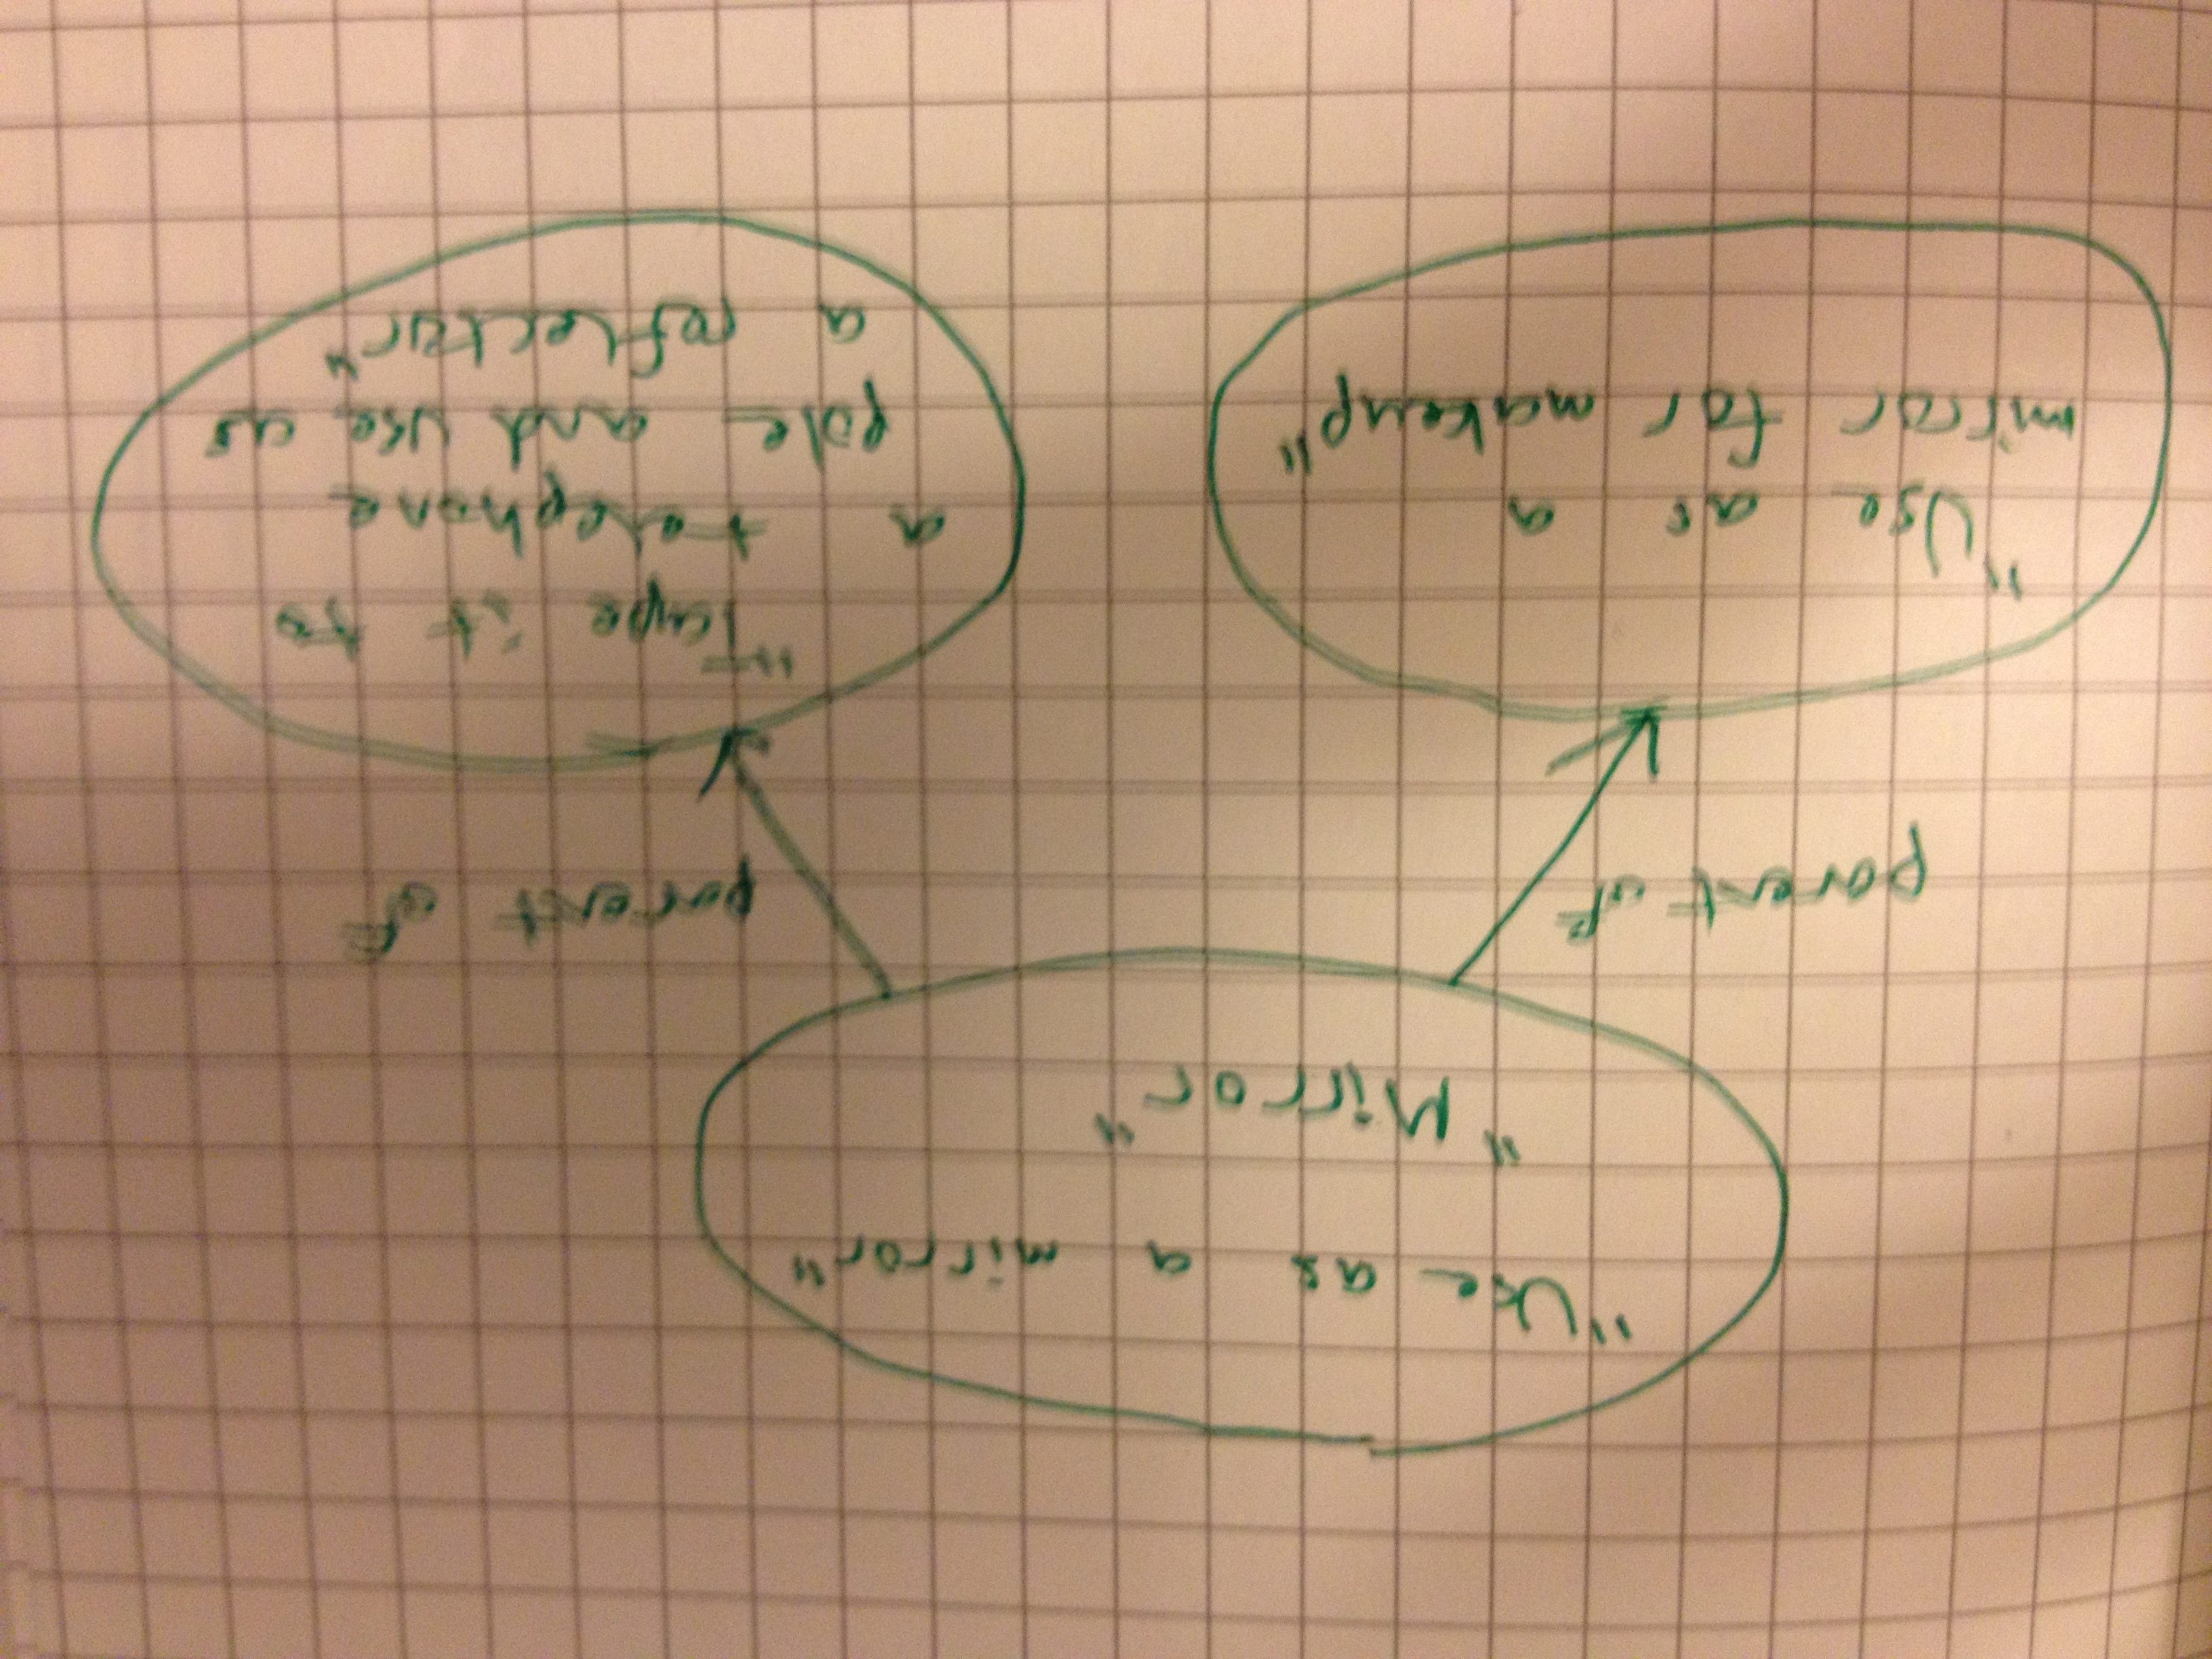
\includegraphics[width=0.9\columnwidth]{sample_category_tree}
\end{figure}

If an idea \emph{A} is a parent of idea \emph{B}, A is a generalization of B: all instances in A are are suitably general to encompass all instances in B. This difference is relative to the ideas in question.

A \emph{question forest} is simply the collection of all category trees generated in response to a particular question. Different trees in a question forest have no special relationship in meaning.

\subsection{Coding}

One researcher coded responses the MP3 problem to produce an idea forest as described above. The MP3 problem was chosen because it was subjectively easiest to distinguish between and categorize ideas.

The clustering algorithm is described in Figure FIG. Instances are added one at a time to the existing idea forest. In brief summary, the root idea that most closely matches the strategy in the instance is selected, and then that root idea and the new instance are compared in generality. This process may be repeated depending on this generality relationship, until instance is either placed in an existing idea or a new idea node is created.

\begin{figure*}[h!]
\small
\begin{verbatim}
for each instance:
  idea_node = new node including instance
  current_node = root of forest
  do:
    best_match = max_similarity(idea_node, current_node.children)

    if best_match.similarity is low or current_node has no children:
      insert idea_node under current_node
      exit do
    else:
      if coverage(idea_node, best_match) == coverage(best_match, idea_node) == high:
        merge idea_node, best_match
        exit do
      else if coverage(idea_node, best_match) == coverage(best_match, idea_node) == low:
        new_parent = new artifical idea node
        insert best_match, idea_node under new_parent
        insert new_parent under current_node
        exit do
      else if coverage(idea_node, best_match) > coverage(best_match, idea_node):
        replace best_match with idea_node in tree
        current_node = idea_node
        idea_node = best_match
      else:
        current_node = best_match
\end{verbatim}
\caption{Manual clustering algorithm}
\label{fig:cluseringalg}
\end{figure*}

The clustering algorithm relies on the human intelligence of the researcher for three key decisions:

\subsubsection{Similarity}
Two ndodes a and b have high similarity if they solve the problem in the same way, and low similarity if their solutions have no common themes. For example, in Figure FIG, "Mirror" and "Tape it to a telephone pole and use as a reflector" have high similarity, as they both solve the problem of using a broken MP3 player by using it to reflect light.

\subsubsection{Coverage}
A node a has high coverage of a node b if the problem solution in a is equal to or an abstraction of the problem solution in b. Coverage is not commutative. To return to the example, "Mirror" has high coverage of "Tape it to a telephone pole and use as a reflector", as the latter is a specific use for a mirror. On the other hand, the latter idea has low coverage of the former.

\subsubsection{Artificial Ideas}
Occasionally, two nodes have high similarity but no coverage. For example, "Use it as a mirror for makeup" and "Tape it to a telephone pole and use as a reflector" use the MP3 player in the same way, but neither is a generalization of the other. In this case, the algorithm appeals to the human coder to provide a lable for a new idea that is a generalization of both.

After completion of the coding algorithm, we were left with an idea forest as described in section SEC.